\section{Hausdorffova míra a Hausdorffova dimenze}\label{sec:hausdorffova-mira-dimenze}

Způsobů, jak definovat dimenzi je celá řada. Zatím jsme společně prozkoumali box-counting dimenzi (resp. některá její pojetí), avšak lze najít více způsobů její definice\footnote{Některé další jsou sepsány např. v \citep[str. 40]{Falconer2014}.}. Pravděpodobně však nejstarším exemplářem svého druhu je tzv. \emph{Hausdorffova dimenze} a s ní související \emph{Hausdorffova míra}, které hrají ve fraktální geometrii velice podstatnou roli. Stále se však budeme zabývat pouze množinami v $\R^n$. Jsou pojmenovány po německém matematikovi \name{Felixi Hausdorffovi} (1868--1942).
% \begin{figure}
%     \centering
%     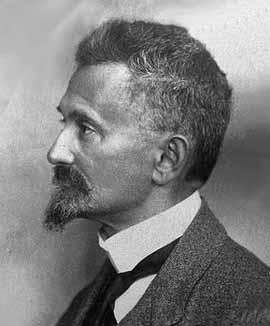
\includegraphics[width=0.4\textwidth]{felix-hausdorff.jpg}
%     \caption[Felix Hausdorff, 1868--1942]{Felix Hausdorff, 1868--1942 (Převzato z \cite{OConnorHausdorff2025})}
% \end{figure}

\subsection{Definice Hausdorffovy míry}\label{subsec:hd-mira-definice}

\begin{definition}\label{def:hd-mira-delta}
    Nechť je dána množina $F\subseteq\R^n$ a $s>0$. Pak pro každé $\delta>0$ definujeme zobrazení
    \[\mathcal{H}_\delta^s(F)=\inf\set{\sum_{i=1}^{\infty}(\diam{F_i})^s\;\middle|\;F\subseteq\bigcup_{i=1}^\infty F_i\;,\;\diam{F_j}\leqslant\delta\;\text{pro}\;1\leqslant j\leqslant n}.\]
\end{definition}
Na první pohled si lze všimnout, že pro $0<\delta_1<\delta_2$ je $\mathcal{H}_{\delta_1}^s(F)\leqslant\mathcal{H}_{\delta_2}^s(F)$. Jinými slovy, pro $\delta\to 0$ hodnota $\mathcal{H}_\delta^s(F)$ klesá. Toto není nikterak těžké si rozmyslet, neboť pro $\delta_1<\delta_2$ existuje $\delta_1$-pokrytí $\mathcal{F}_1$, takové, že je podpokrytím $\delta_2$-pokrytí $\mathcal{F}_2$ množiny $F$, tedy $\mathcal{F}_1\subseteq\mathcal{F}_2$. To znamená, že
\begin{align*}
    \mathcal{H}_{\delta_1}^s(F)&=\inf\set{\sum_{U\in\mathcal{F}_1}(\diam{U})^s\;\middle|\;\text{$\mathcal{F}_1$ je $\delta_1$-pokrytí}}\\
    &\leqslant\inf\set{\sum_{U\in\mathcal{F}_2}(\diam{U})^s\;\middle|\;\text{$\mathcal{F}_2$ je $\delta_2$-pokrytí}}=\mathcal{H}_{\delta_2}^s(F).
\end{align*}
Zároveň je z definice \ref{def:hd-mira-delta} zjevné, že $\mathcal{H}_\delta^s(F)\geqslant 0$.

\todo{Doplnit důkaz, že Hausdorffova míra je mírou}